% Figure 1 for FORGE paper: input (network + description) -> FORGE -> output
% Compile: pdflatex fig1_pipeline.tex
\documentclass[tikz,border=2pt]{standalone}
\usepackage[T1]{fontenc}
\usepackage{courier}
\usepackage{amssymb}
\usepackage[scaled=0.96]{helvet}
\renewcommand{\familydefault}{\sfdefault}
\usetikzlibrary{positioning,arrows.meta,calc}

% ---------- palette ----------
\definecolor{panelbg}{HTML}{F6F8FB}
\definecolor{panelbd}{HTML}{D7DEE8}
\definecolor{ink}{HTML}{1F2A37}
\definecolor{muted}{HTML}{5B6B7C}
\definecolor{blue}{HTML}{2B6CB0}
\definecolor{bluebg}{HTML}{EBF2FA}
\definecolor{green}{HTML}{2F855A}
\definecolor{greenbg}{HTML}{ECF7F0}
\definecolor{red}{HTML}{C0392B}
\definecolor{codebg}{HTML}{EEF1F6}
\definecolor{clubA}{HTML}{5A67D8}
\definecolor{clubB}{HTML}{ED8936}
\definecolor{clubC}{HTML}{319795}

\begin{document}
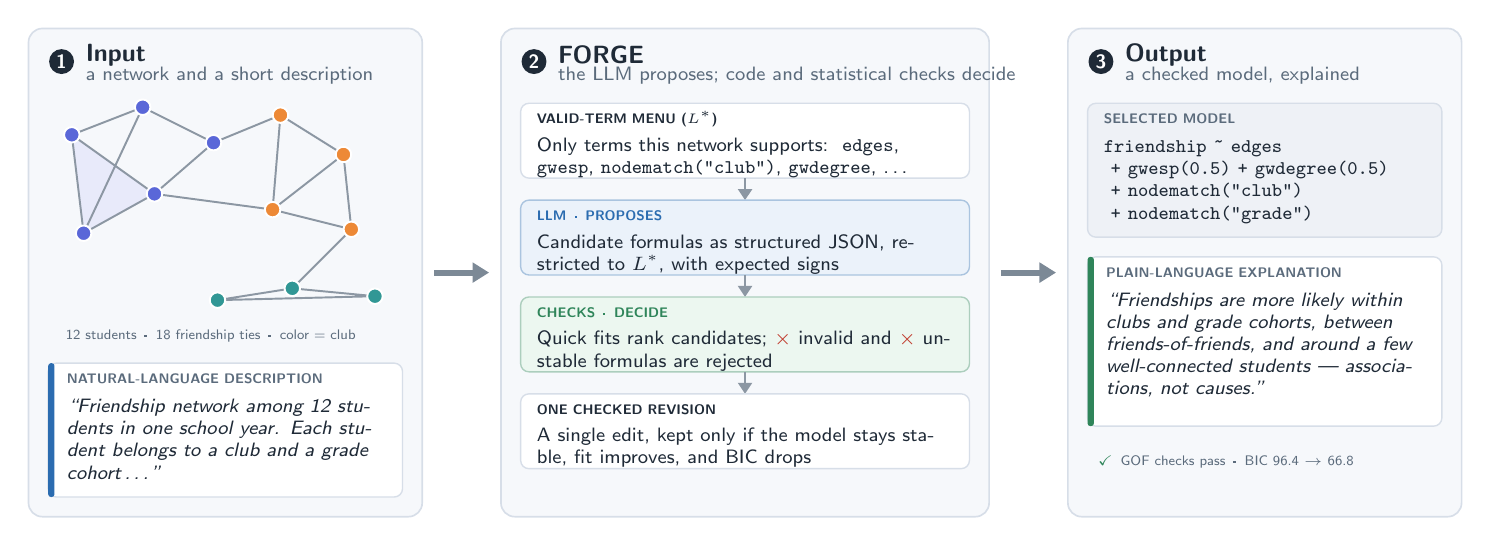
\begin{tikzpicture}[
  x=1cm,y=1cm,
  panel/.style={draw=panelbd,fill=panelbg,rounded corners=5pt,line width=0.6pt},
  card/.style={draw=panelbd,fill=white,rounded corners=3pt,line width=0.5pt},
  badge/.style={circle,fill=ink,text=white,inner sep=0pt,minimum size=9pt,font=\bfseries\scriptsize},
  ptitle/.style={font=\bfseries\small,text=ink,anchor=west,inner sep=0pt},
  psub/.style={font=\scriptsize,text=muted,anchor=west,inner sep=0pt},
  taglab/.style={font=\bfseries\tiny,anchor=west,inner sep=0pt},
  body/.style={font=\scriptsize,text=ink,anchor=north west,inner sep=0pt,align=left},
  dotA/.style={circle,fill=clubA,draw=white,line width=0.7pt,inner sep=0pt,minimum size=5.6pt},
  dotB/.style={circle,fill=clubB,draw=white,line width=0.7pt,inner sep=0pt,minimum size=5.6pt},
  dotC/.style={circle,fill=clubC,draw=white,line width=0.7pt,inner sep=0pt,minimum size=5.6pt},
  netedge/.style={draw=muted!70,line width=0.7pt},
  bigarrow/.style={-{Triangle[length=6pt,width=7pt]},line width=2.2pt,draw=muted!80},
  rowarrow/.style={-{Triangle[length=4pt,width=5pt]},line width=1pt,draw=muted!70}
]

% ============================================================ PANEL 1: INPUT
\draw[panel] (0,0) rectangle (5.0,6.2);
\node[badge] at (0.42,5.78) {1};
\node[ptitle] at (0.72,5.86) {Input};
\node[psub]   at (0.72,5.60) {a network and a short description};

% --- network drawing ---
\begin{scope}[shift={(0.25,2.55)}]
  % edges first
  \coordinate (n0) at (0.45,1.05);
  \coordinate (n1) at (0.30,2.30);
  \coordinate (n2) at (1.35,1.55);
  \coordinate (n3) at (1.20,2.65);
  \coordinate (n4) at (2.10,2.20);
  \coordinate (n5) at (2.95,2.55);
  \coordinate (n6) at (3.75,2.05);
  \coordinate (n7) at (2.85,1.35);
  \coordinate (n8) at (3.85,1.10);
  \coordinate (n9) at (3.10,0.35);
  \coordinate (n10) at (4.15,0.25);
  \coordinate (n11) at (2.15,0.20);
  % subtle highlight: one closed triangle (triadic closure) inside club A
  \fill[clubA!14] (n0)--(n1)--(n2)--cycle;
  \draw[netedge] (n0)--(n1) (n0)--(n2) (n1)--(n2) (n1)--(n3) (n2)--(n4)
                 (n3)--(n4) (n0)--(n3) (n5)--(n6) (n5)--(n7) (n6)--(n7)
                 (n6)--(n8) (n7)--(n8) (n9)--(n10) (n9)--(n11) (n10)--(n11)
                 (n4)--(n5) (n8)--(n9) (n2)--(n7);
  \node[dotA] at (n0) {}; \node[dotA] at (n1) {}; \node[dotA] at (n2) {};
  \node[dotA] at (n3) {}; \node[dotA] at (n4) {};
  \node[dotB] at (n5) {}; \node[dotB] at (n6) {}; \node[dotB] at (n7) {};
  \node[dotB] at (n8) {};
  \node[dotC] at (n9) {}; \node[dotC] at (n10) {}; \node[dotC] at (n11) {};
\end{scope}
% legend / stats line
\node[font=\tiny,text=muted,anchor=west] at (0.35,2.30)
  {12 students \,\textperiodcentered\, 18 friendship ties \,\textperiodcentered\, color = club};

% --- description quote card ---
\draw[card] (0.25,0.25) rectangle (4.75,1.95);
\fill[blue,rounded corners=1pt] (0.25,0.25) rectangle (0.33,1.95);
\node[taglab,text=muted] at (0.48,1.75) {NATURAL-LANGUAGE DESCRIPTION};
\node[body,text width=4.0cm,font=\scriptsize\itshape] at (0.48,1.50)
  {``Friendship network among 12 students in one school year. Each student
    belongs to a club and a grade cohort\,\dots''};

% ============================================================ ARROW 1
\draw[bigarrow] (5.15,3.1) -- (5.85,3.1);

% ============================================================ PANEL 2: FORGE
\draw[panel] (6.0,0) rectangle (12.2,6.2);
\node[badge] at (6.42,5.78) {2};
\node[ptitle] at (6.72,5.86) {FORGE};
\node[psub]   at (6.72,5.60) {the LLM proposes; code and statistical checks decide};

% row 1 : valid terms
\draw[card] (6.25,4.30) rectangle (11.95,5.25);
\node[taglab,text=ink] at (6.45,5.05) {VALID-TERM MENU ($L^{*}$)};
\node[body,text width=5.3cm] at (6.45,4.82)
  {Only terms this network supports:\ \ \texttt{edges}, \texttt{gwesp},
   \texttt{nodematch("club")}, \texttt{gwdegree}, \dots};
\draw[rowarrow] (9.10,4.30) -- (9.10,4.02);

% row 2 : LLM proposes
\draw[card,fill=bluebg,draw=blue!40] (6.25,3.07) rectangle (11.95,4.02);
\node[taglab,text=blue] at (6.45,3.82) {LLM \,\textperiodcentered\, PROPOSES};
\node[body,text width=5.3cm] at (6.45,3.59)
  {Candidate formulas as structured JSON, restricted to $L^{*}$, with expected signs};
\draw[rowarrow] (9.10,3.07) -- (9.10,2.79);

% row 3 : checks decide
\draw[card,fill=greenbg,draw=green!40] (6.25,1.84) rectangle (11.95,2.79);
\node[taglab,text=green] at (6.45,2.59) {CHECKS \,\textperiodcentered\, DECIDE};
\node[body,text width=5.3cm] at (6.45,2.36)
  {Quick fits rank candidates; \textcolor{red}{$\times$}~invalid and
   \textcolor{red}{$\times$}~unstable formulas are rejected};
\draw[rowarrow] (9.10,1.84) -- (9.10,1.56);

% row 4 : one checked revision
\draw[card] (6.25,0.61) rectangle (11.95,1.56);
\node[taglab,text=ink] at (6.45,1.36) {ONE CHECKED REVISION};
\node[body,text width=5.3cm] at (6.45,1.13)
  {A single edit, kept only if the model stays stable, fit improves, and BIC drops};

% ============================================================ ARROW 2
\draw[bigarrow] (12.35,3.1) -- (13.05,3.1);

% ============================================================ PANEL 3: OUTPUT
\draw[panel] (13.2,0) rectangle (18.2,6.2);
\node[badge] at (13.62,5.78) {3};
\node[ptitle] at (13.92,5.86) {Output};
\node[psub]   at (13.92,5.60) {a checked model, explained};

% selected model (code card)
\draw[card,fill=codebg] (13.45,3.55) rectangle (17.95,5.25);
\node[taglab,text=muted] at (13.65,5.05) {SELECTED MODEL};
\node[body,font=\scriptsize\ttfamily,text width=4.2cm] at (13.65,4.78)
  {friendship \char126\ edges\\
   \ + gwesp(0.5) + gwdegree(0.5)\\
   \ + nodematch("club")\\
   \ + nodematch("grade")};

% plain-language explanation
\draw[card] (13.45,1.15) rectangle (17.95,3.30);
\fill[green,rounded corners=1pt] (13.45,1.15) rectangle (13.53,3.30);
\node[taglab,text=muted] at (13.68,3.10) {PLAIN-LANGUAGE EXPLANATION};
\node[body,text width=4.05cm,font=\scriptsize\itshape] at (13.68,2.85)
  {``Friendships are more likely within clubs and grade cohorts, between
    friends-of-friends, and around a few well-connected students ---
    associations, not causes.''};

% evidence chip
\node[font=\tiny,text=muted,anchor=west] at (13.45,0.70)
  {\textcolor{green}{\bfseries\checkmark}\, GOF checks pass
   \,\textperiodcentered\, BIC 96.4 $\rightarrow$ 66.8};

\end{tikzpicture}
\end{document}
